
\newcommand{\imagw}[3]{
  \begin{figure}[!hbt]
    \centering
    \includegraphics[width=#1]{#2}
    \caption{#3}
    \label{fig:#2}
  \end{figure}
}

\newcommand{\imag}[2]{\imagw{16cm}{#1}{#2}}

\chapter{Setup for spatio-angular illumination}
\begin{summary}
  We build something
\end{summary}

\nomenclature{MEMI}{Micro-mirror enhanced micro-imaging. EU FP7
  project reference 215597.}
\section{Overview}
\figref{fig:memi-simple} shows a simplified schematic of our optical
system. A laser light source is scrambled by a rotating microlens
array and mixed in an integrating tunnel with a quadratic cross
section. The uniform light distribution from the end of the tunnel is
imaged into the specimen. Two spatial light modulators allow to modify
the light intensity and angular distribution of the light within the
sample.

\begin{figure}[!hbt]
  \centering
  \def\svgscale{1.5}
  \input{memi-simple.eps_tex}
  \caption{Simplified schematic of the MEMI system. Light coming from
    the source is homogenized in an integrating tunnel. The light then
    traverses two spatial light modulators. The first of which (MMA)
    is imaged into the back focal plane of the objective and the
    second (LCoS) into the sample.}
  \label{fig:memi-simple}
\end{figure}

\figref{fig:hourglass-all} visualizes how our optical system improves
sample illumination. If the LCoS illuminates one in-focus
bead\footnote{Note that the LCoS acts as a Fourier filter on the
  information coming from the MMA. Therefor if all but a single pixel
  of the LCoS block the light, no angular control is possible.}, the
MMA can be used to prevent exposure of the out of focus bead in
\figref{fig:hourglass-all}~(a). Not exciting the out-of-focus bead has
two advantages:
\begin{enumerate}
\item There is less background light in the camera image, leading to a
  clearer image of the in-focus information. It would be possible to
  computationally distinguish and subtract out-of-focus light by
  structured illumination methods but these methods will not remove
  the poisson distributed photon noise of the out-of-focus light.
\item Not exciting the out-of-focus areas is especially important for
  biological specimen in order to reduce the phototoxicity of the
  imaging.
\end{enumerate}
If an extended in-focus area should be imaged
(\figref{fig:hourglass-all}~(d)). Then multiple exposures, each with
different patterns on LCoS and MMA, can be combined into an image of
the in-focus information with minimal exposure of out-of-focus
fluorophores.

This technique requires prior knowledge about the fluorophore
distribution in the sample. In 3D time lapse imaging of developing
embryos a good estimate is available when the stacks are acquired with
high enough temporal resolution. Opto-genetics experiments can be
designed such, that the 3D distribution of neurons is known before
single neurons are triggered by light without exposing its neighbours.

\begin{figure}[!hbt]
  \centering
  \def\svgscale{.43}
  \input{hourglass-all.eps_tex}
  \caption{{\bf (a)} Two fluorescent beads are illuminated by all
    angles that an objective can deliver. The sharp image of the
    in-focus bead is deteriorated by blurry fluorescence of the out of
    focus bead. {\bf (b)} Angular control allows selective
    illumination of the in-focus bead and results in a better image on
    the camera. {\bf (c)} Angular control is insufficient, when an
    extended in focus area is illuminated. {\bf (d)} However,
    simultaneous spatial and angular control allows sequential
    excitation of the in-focus beads while excluding the out of focus
    bead.}
  \label{fig:hourglass-all}
\end{figure}

\section{Details}

In the real system the spatial light modulators are reflective. 
Also both displays are not direct intensity modulators.


\figref{fig:setup-gimp} shows a schematic of the light path in
the combined angular and spatial control system. The distance between
either source or MMA and the lens L1 is equal to the focal distance ofo
L1. Therefor if all mirrors of the MMA are flat, an image of the
source is formed in the plane of the aperture B1. The size of the
aperture is chosen to transmit just this image. When mirrors of the
MMA are tilted, they will slightly deflect the light, so that it no
longer passes through the aperture.  In the schematic the left half of
the MMA mirrors are tilted. Therefore the right part of the back focal
plane of the objective L5 is not illuminated and the light pattern
that excites the fluorophores in the sample is only half of the
conventional "hourglass" double cone.

The lenses L2 and L3 relay the image of the source from B1 into the
LCoS plane.  The incoming light is linearly polarized and its electric
field vibrates in the plane of the paper. Depending its state (on or
off) the LCoS pixel can rotate the polarization of the returning
light, so that it is reflected towards the objective L5 by the
polarizing beam splitter PBS.

fig:memi-sketch


In the front focal plane of the objective L5 an image of the pattern
on the LCoS is formed. Excited fluorophores emit fluorescence photons
of which a certain solid angle is collected by the objective L5
(depicted as green ray bundle). The dichroic beam splitter D1 reflects
these photons down. The tube lens L4 forms an image of the fluorescent
object in the camera plane.

\begin{figure}[!hbt]
  \centering
  \def\svgscale{2}
  \input{memi-real.eps_tex}
  \caption{Schematic of the light path through our
  microscope. M1 and M2 are mirrors.  L1, L2, L3, L4 and L5 are
  lenses. B1 is an adjustable circular aperture. PBS is a polarizing
  beam splitter. D1 is a dichroitic beam splitter.}
  \label{fig:memi-real}
\end{figure}


\imag{setup-photo-blueprint}{The widefield epi-fluorescent microscope
  with attached illumination head. The positions of the two spatial
  light modulators (Micro mirror array (MMA) and liquid crystal on
  silicon display (LCoS)) are indicated.}

\imag{mma}{{\bf left:} Scanning electron microscope image of the
  micro-mirror array (MMA).  The pixel pitch of the device is
  \unit[0.016]{mm}. The hinges for the tilt movement and the
  electrodes are clearly visible. {\bf middle:} Optical reflective
  microscope image of the MMA. {\bf right:} exaggerated rendering of
  how a 8x8 checker board pattern would be displayed on the device.}

\imagw{8cm}{optimization}{bnla lba}

\begin{figure}[!hbt]
  \centering
  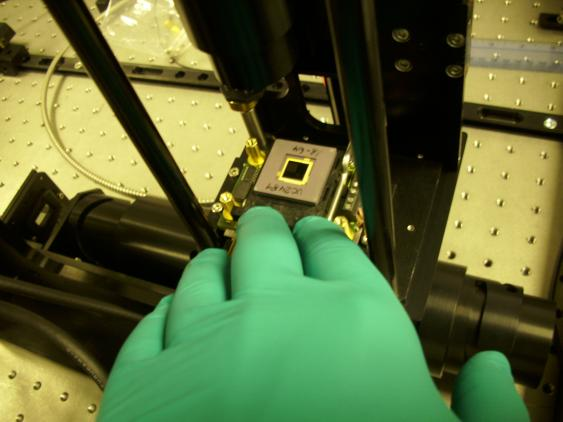
\includegraphics[width=7cm]{mma-plain}
  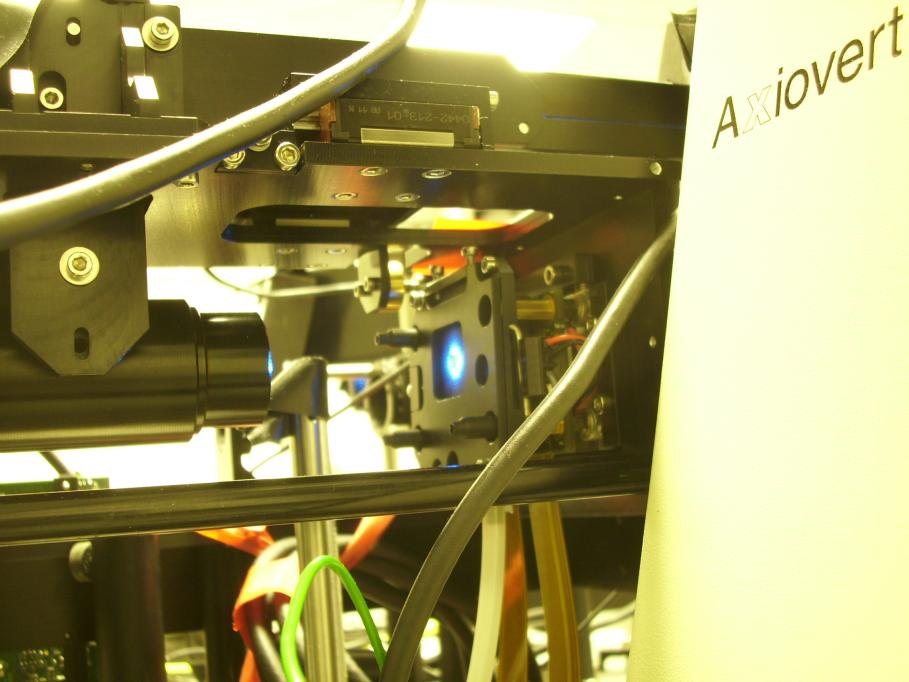
\includegraphics[width=7cm]{mma-ill}
  \caption{{\bf left:} Micro mirror array chip during installation of
    the optics. {\bf right:} Illuminated micro mirror array in the
    aligned system.}
  \label{fig:mma-closeup}
\end{figure}

\begin{figure}[!hbt]
  \centering
  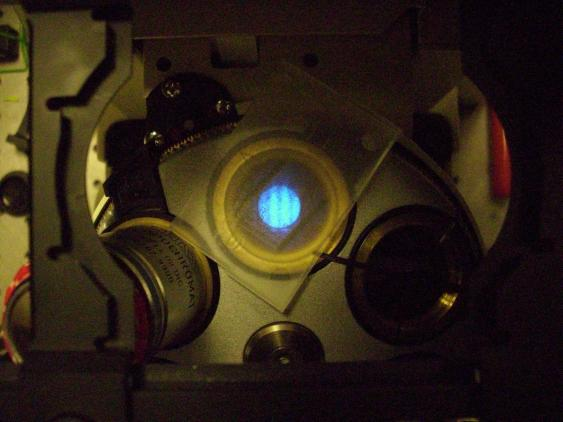
\includegraphics[width=7cm]{bfp1}
  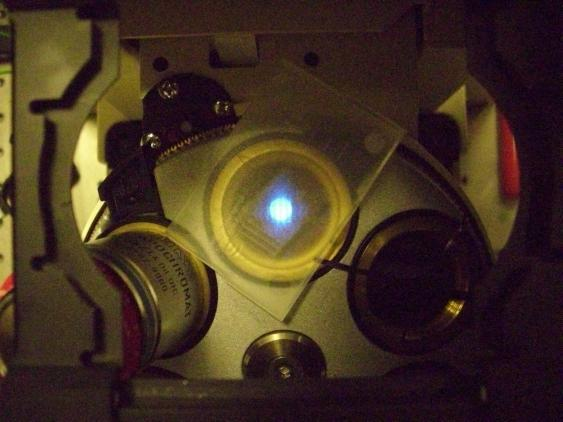
\includegraphics[width=7cm]{bfp2}
  \caption{Images of the micro mirror array in the back focal plane
    with different settings of the variable tubelens.}
  \label{fig:mma-closeup}
\end{figure}

\imagw{5cm}{lcos}{lcos}

